\chapter{Copulas}\label{ch:4}

In this chapter, we explore how well the dependence among systems is modeled by the copulas, regardless of their marginal distributions. The methodologies used in this chapter are analogous to Chapter \ref{ch:3}. In this thesis, we focus specifically on the case of only two systems, as done in \cite{Urbano2019}. This means that we deal with the specific case of \textit{bi-variate} copulas. 

\section{Experiments}

In order to measure the goodness-of-fit of the copulas, we once again utilize the split-half approach, as shown in Figure \ref{fig:diag6}. The approach is slightly different in the case of copulas, compared to the case of the margins, for two reasons. Firstly, the distributions are joint instead of univariate. Joint distributions are visually represented as surfaces instead of curves. For this reason, $\Delta_\text{obs}$ and $\Delta_\text{exp}$ are computed by measuring the volume between surfaces, as opposed to the area between curves. Secondly, the scores need to be converted to pseudoscores, as we previously discussed (see Figure \ref{fig:sim-diag}). 

\begin{figure}[h]
	\centering	
	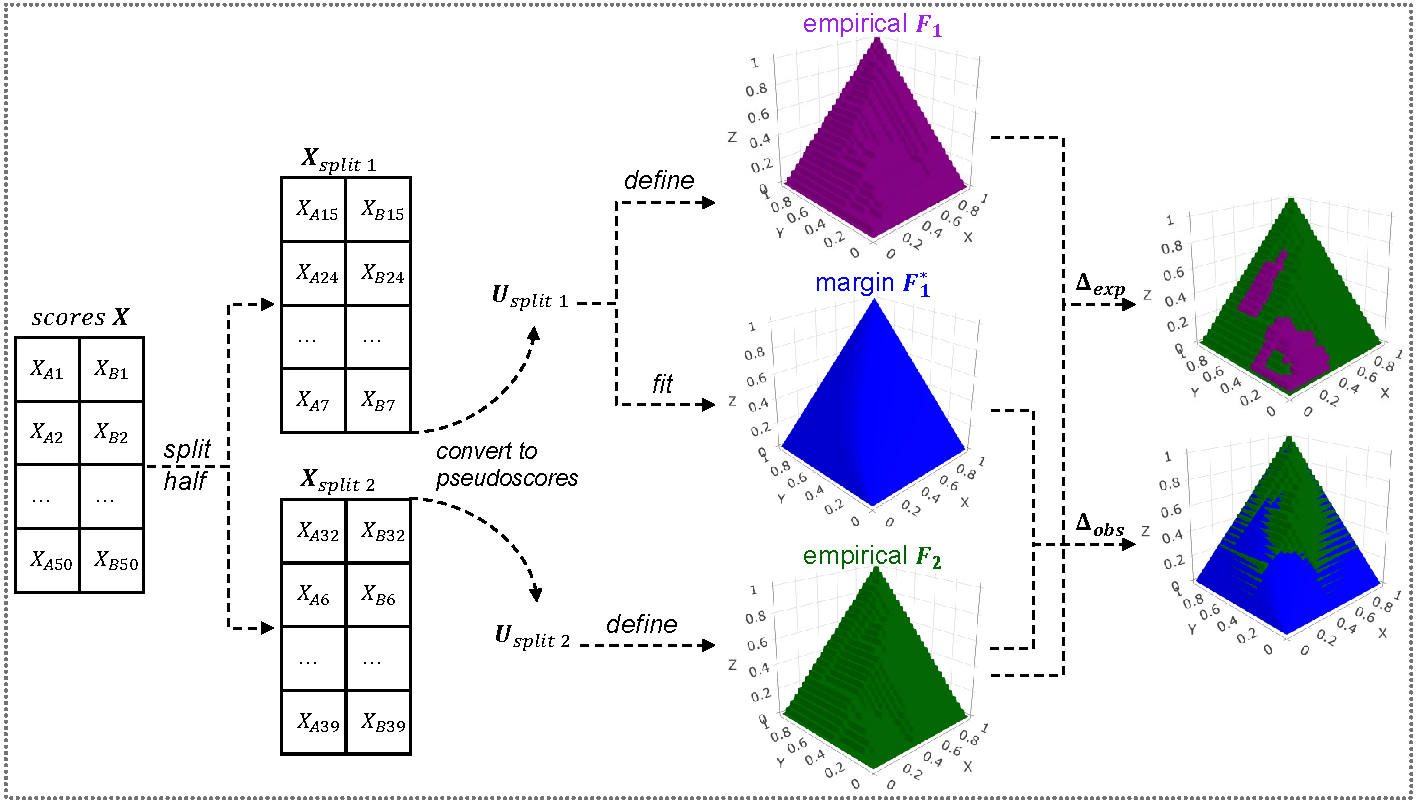
\includegraphics[width=1.0\linewidth]{../diagrams/diag6}
	\caption{Diagrammatic representation of the split-half approach for the case of bi-variate copula models. The $\Delta_\text{obs}$ and $\Delta_\text{exp}$ are computed by measuring the volume between the two surfaces.}
	\label{fig:diag6}
\end{figure}

\clearpage

Our primary objective is to measure how well can copulas capture the dependence between two given systems. To this end, for each effectiveness measure, we select two random systems from a random collection and perform the aforementioned split-half approach using the scores of those systems on the entire set of 50 topics. Once again, a total of \num{250000} splits were performed; \num{50000} for each effectiveness measure. This amount of splits seems to be sufficient, judging from the narrow confidence intervals we obtain for most of our results. The data collections we used are the same as those in the case of the margins (Table \ref{tab:dataset-descriptive-stats}). For each split, we calculate a corresponding $\Delta_\text{exp}$. Then, using the data in the first half of the split, we fit all copulas (according to Table \ref{tab:fams}), and compute their corresponding $\Delta_\text{obs}$. 

Figure \ref{fig:copula-example-split} shows the $\Delta_\text{obs}$ (left) and $\Delta_\text{exp}$ (right), in one example random split. The approach we use for computing these $\Delta_\text{obs}$ and $\Delta_\text{exp}$ values, is to average the absolute differences between the two surfaces (in the Z-axis), across $100x100$ equally spaced points. In this example, the best copula model according to AIC, was a Joe copula, that measured $\Delta_\text{obs}=0.02$. The expected $\Delta$ was measured at 0.026.

\begin{figure}[t]
	\centering
	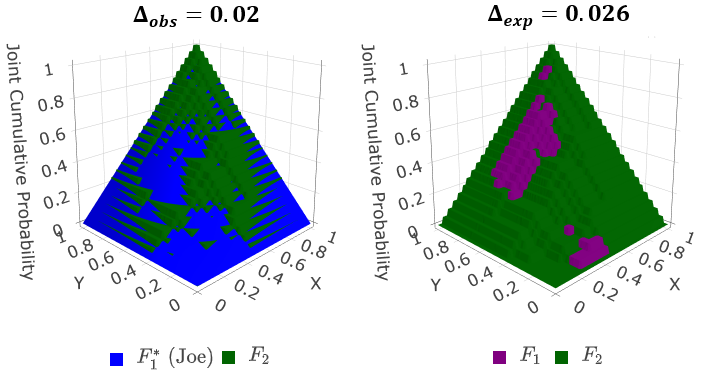
\includegraphics[width=0.7\linewidth]{copulas/6.png}
	\caption{Visualization of $\Delta_{\text{obs}}$ (left) and $\Delta_{\text{exp}}$ (right) for an example random split that was performed on the AP scores of systems 16 and 43, on the 50 topics of the Ad-hoc 2007 test collection. Each $\Delta$ is the volume between two surfaces.}
	\label{fig:copula-example-split}
\end{figure}

In Figure \ref{fig:copulas-splithalf-plot-1&2b}, we report the results across all \num{250000} random splits, separately for each effectiveness measure and copula family. All model selections were made according to AIC. In the right plot, we have removed the copulas BB1 and BB6, to make it easier to view the results, due to the fact that those copulas are outliers in terms of their GoF. This occurrence is simply due to chance. In those particular splits, where BB1 or BB6 are selected, the $\Delta_{\text{exp}}$ values are much lower than usual. This implies that in those particular random splits, the two data halves are much more similar than usual. In those cases, the GoF value is low, due to the division with $\Delta_{\text{exp}}$. This phenomenon is mostly inconsequential, because, as we can see in Table \ref{tab:bb1&6-freq}, the copulas BB1 and BB6 are almost never selected. Overall, the copula families measure a $\Delta_{\text{obs}}$ that is strictly larger than $\Delta_{\text{exp}}$, on average. To make it easier to interpret the results, looking at the right plot, we see that GoF is mostly negative, at around -0.23, which implies that, on average, we measure $\Delta_{\text{obs}}$ values that are about 23\% higher than the expectation. This is somewhat higher than we would ideally wish for, although it is still within reason. Moreover, in contrast to the case of the margins, we do not detect any obvious outliers, as the performance appears to be spread somewhat evenly across the different copula models.

Figure \ref{fig:copulas-splithalf-plot-3}, shows the frequency with which each candidate copula family is selected, when the models are fitted on \textit{i)} 25, as well as \textit{ii)} 50 topics. It appears that the copulas are selected somewhat similarly between these two cases. This adds a degree of confidence regarding the accuracy of our estimates of goodness-of-fit. Moreover, it reaffirms the idea that IR data are quite complex, since all candidate families get selected, and no particular family gets chosen with a disproportionately higher frequency than the rest. In other words, this implies that a variety of copula models is required, to describe IR data.

\begin{figure}[!t]
	\centering	
	\begin{subfigure}[t]{.42\textwidth}
		\centering
		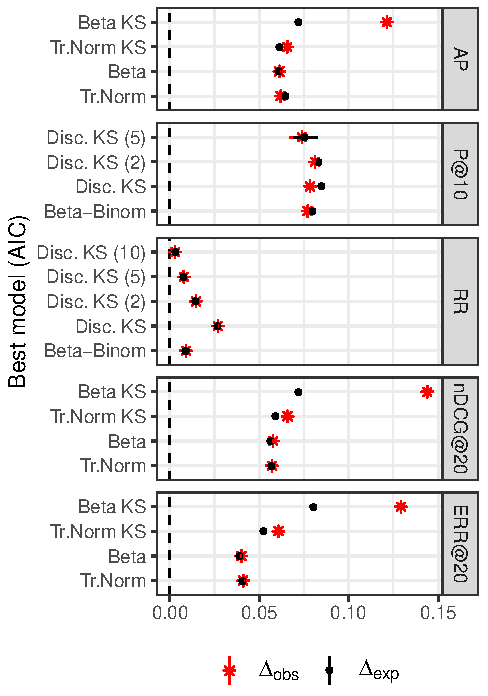
\includegraphics[scale=0.84,valign=t]{copulas/splithalf_n250000_fig1}
	\end{subfigure}%
	\begin{subfigure}[t]{.42\textwidth}
		\centering
		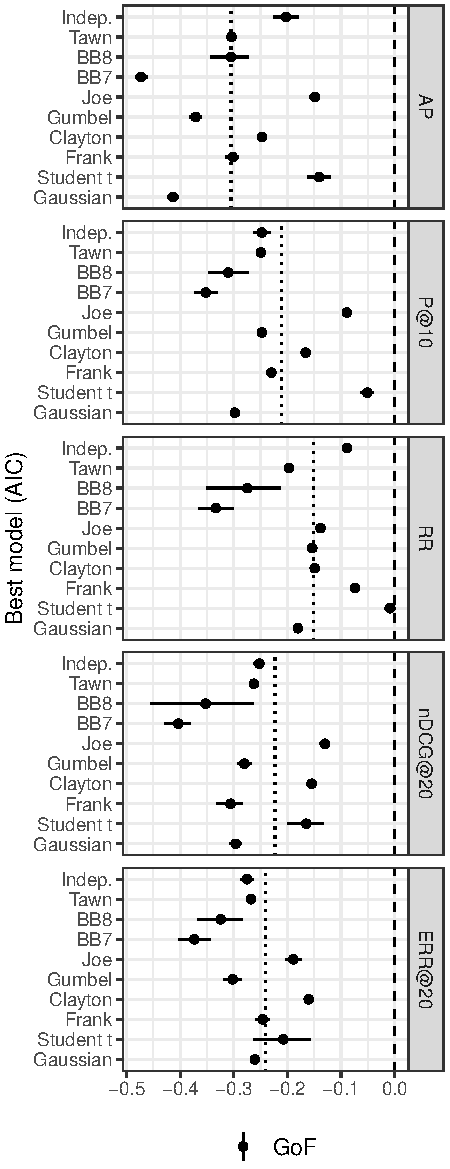
\includegraphics[scale=0.84,valign=t]{copulas/splithalf_n250000_fig2b}
	\end{subfigure}
	\caption{How well does each copula family perform, when it is selected by AIC? In the right plot, outliers BB1 and BB6, are excluded from the list of candidates.}
	\label{fig:copulas-splithalf-plot-1&2b}
\end{figure}

\begin{figure}[!t]
	\centering	
	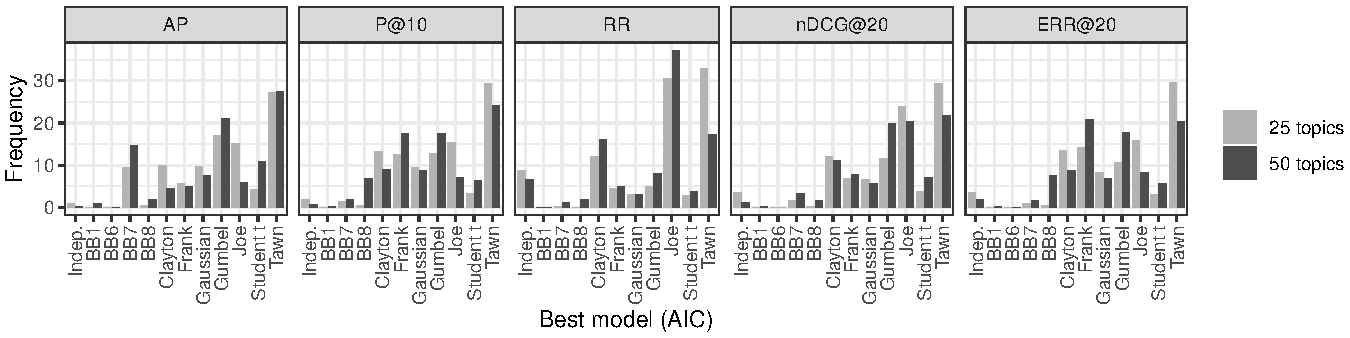
\includegraphics[width=1\linewidth]{copulas/splithalf_n250000_fig3}
	\caption{Frequency with which each candidate copula family is selected by AIC. We consider the case where models are fitted on 25 and 50 topics respectively.}
	\label{fig:copulas-splithalf-plot-3}
\end{figure}

\begin{table}[t]
	\centering
	\begin{tabular}{c c c c} % middle column is all italic
		\toprule
		\multicolumn{2}{c}{\textbf{BB1}} & \multicolumn{2}{c}{\textbf{BB6}} \\ 
		\textit{25 topics} & \textit{50 topics} & 25 \textit{topics} & \textit{50 topics} \\
		\midrule
		%		AP          & 0.088  & 0.881  & 0.012   & 0.008 \\ 
		%		P@10        & 0.006  & 0.302  & 0       &  0     \\
		%		RR          & 0      & 0.0841 & 0       &  0     \\
		%		nDCG@20     & 0.038  & 0.171  & 0.008   &  0    \\
		%		ERR@20      & 0.044  & 0.352  & 0.026   & 0.08  \\
		%		\midrule
		0.04\% & 0.36\%  & 0.01\% & 0.02\% \\
		\bottomrule
	\end{tabular}
	\caption{How often is BB1 and BB6 selected by AIC? We consider the case where models are fitted on 25 and 50 topics respectively.}
	\label{tab:bb1&6-freq}
\end{table}

One possible explanation for these results could be that our list of candidate copulas contains an insufficient selection of asymmetric copula families. In Figure \ref{fig:copulas-splithalf-plot-3}, we see that the Tawn copula is selected with the most frequency, almost consistently across all metrics. The Tawn copula is actually the \textit{only} asymmetric copula that is included in our list of candidates. It could be the case that asymmetric copulas capture the dependence among systems well, but there is simply not a diverse enough selection of them in our list of candidates to cover all scenarios. Figure \ref{fig:skewness} illustrates that the distribution of per-topic score differences, in the case of actual TREC data, is often asymmetric. Furthermore, it shows that only the Tawn copula is able to produce skewed distributions. In many cases, the skewness that is present in actual TREC data is not maintained in the simulated data. This supports the idea that the simulation could potentially be improved by expanding the list of candidates with more asymmetric copulas.

\begin{figure}[t]
	\centering	
	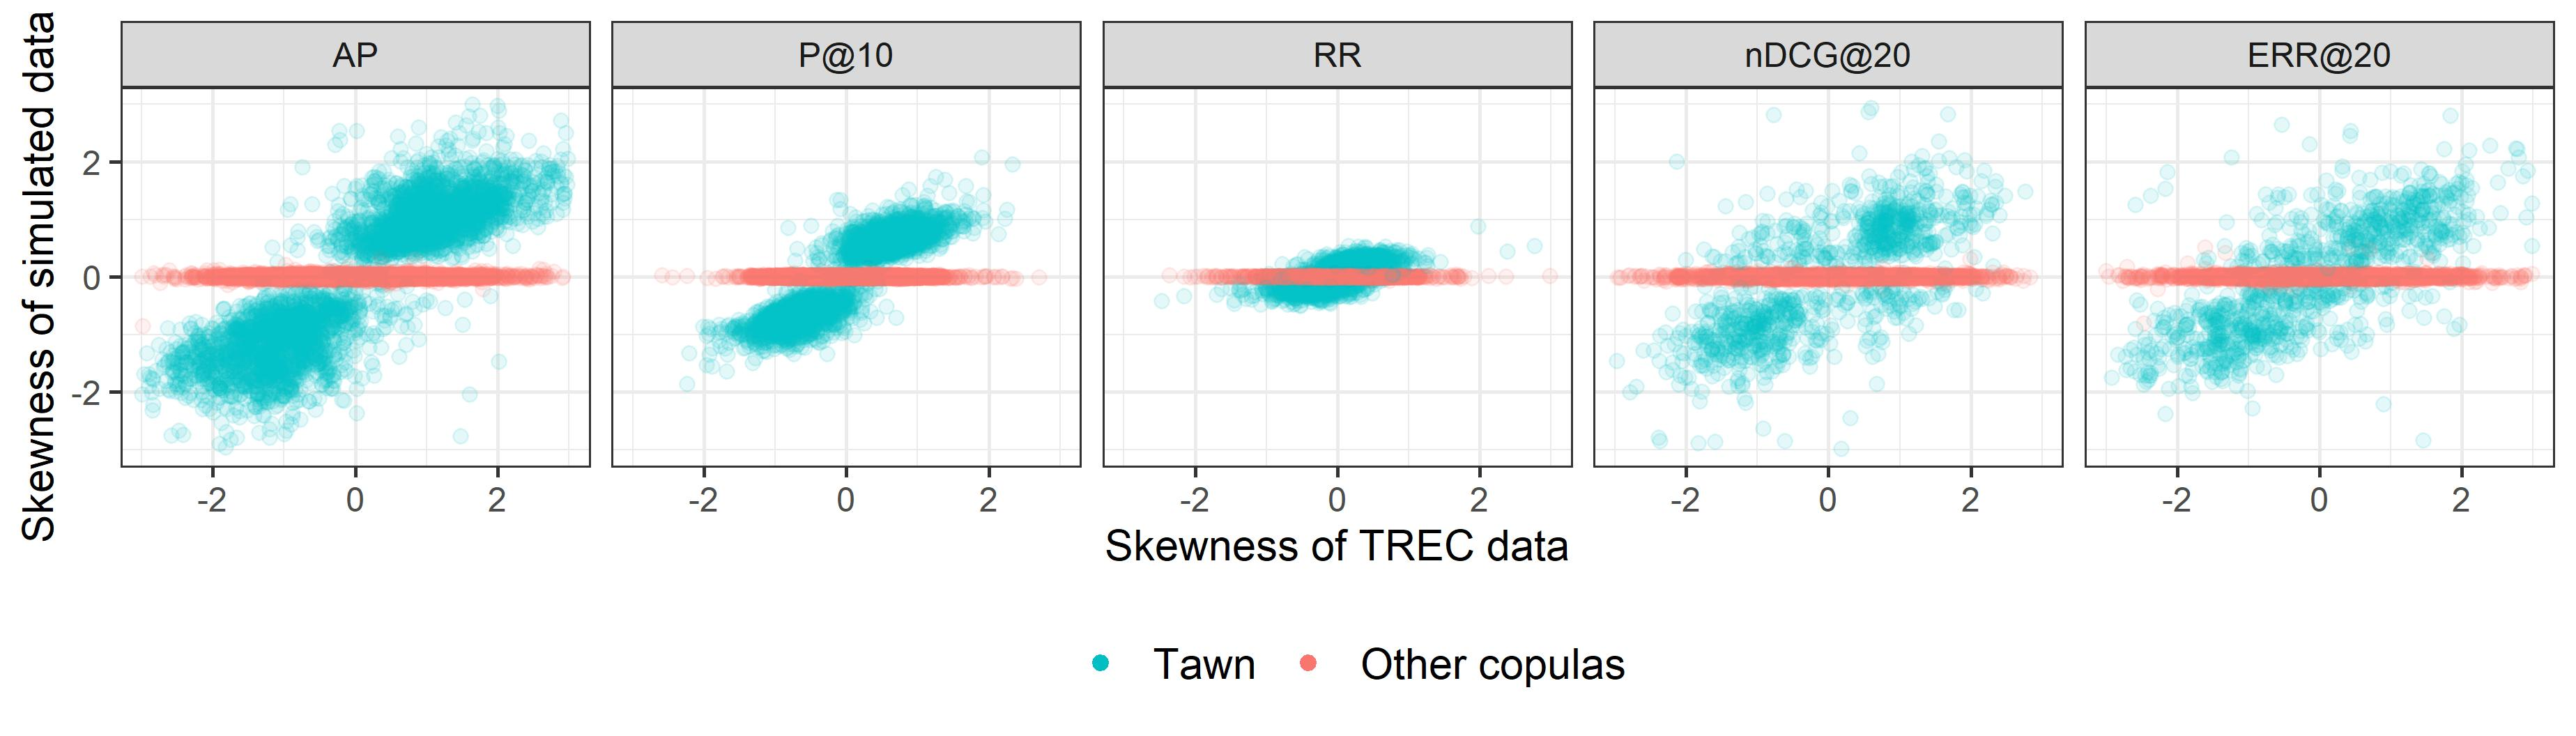
\includegraphics[width=1\linewidth]{copulas/skewness}
	\caption{(Copy of Figure 5 from \cite{Urbano2021}.) Skewness of the distribution of per-topic score differences, in the case of actual TREC data, compared to simulated data. Only the Tawn copula is able to produce skewed distributions.}
	\label{fig:skewness}
\end{figure}

\subsection{Comparing Model Selection Criteria}

In view of our findings regarding the lower than expected goodness-of-fit of the copula models, it is meaningful to experiment with alternative ways of selecting models, in an attempt to improve the overall performance. It is possible that some model selection criteria, other than AIC, might be able to select the candidate copulas more optimally.

In Figure \ref{fig:copulas-splithalf-plot-4}, we compare the performance of LL, AIC, BIC, as well as our proposed criterion SHC, where we set its parameter for the number of splits at $n=10$. This comparison was performed on the same \num{250000} random splits that we previously created. Interestingly, our criterion selects the models more optimally, consistently across all effectiveness measures; in both absolute terms ($\Delta_{\text{obs}}$), and terms relative to the expectation (GoF). Although, all criteria perform quite similarly. AIC appears to be the second best criterion, followed by BIC, and finally by LL. Overall, selecting the copulas with SHC compared to AIC, improves the GoF from approximately $-0.23$ to $-0.19$. Because a variety of criteria was compared, this implies that in order to further improve the goodness-of-fit by a significant amount, beyond the use of SHC, would likely require to enrich the list of candidates with additional copula families. These results further support the hypothesis we previously proposed, regarding the lack of asymmetric copulas in the list of candidates. 

\begin{figure}[t]
	\begin{subfigure}{1\textwidth}
		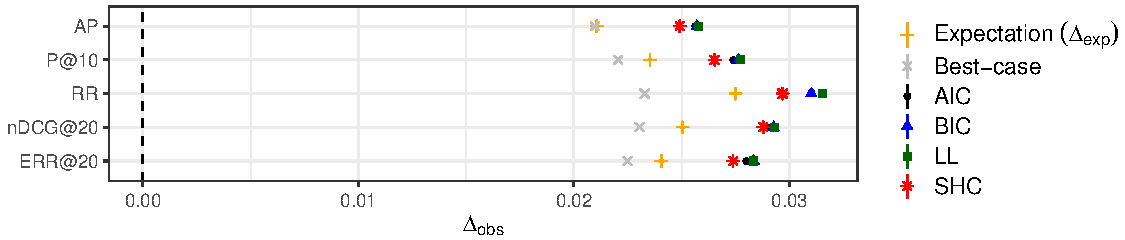
\includegraphics[width=1\linewidth]{copulas/splithalf_n250000_fig4}
	\end{subfigure} \newline
	\begin{subfigure}{1\textwidth}
		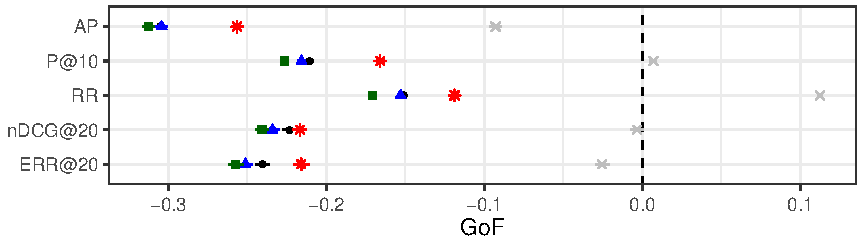
\includegraphics[width=0.768\linewidth]{copulas/splithalf_n250000_fig4b}
	\end{subfigure}
	\caption{Comparison of the model selection criteria, in terms of overall mean $\Delta_{\text{obs}}$ and GoF that is measured.}
	\label{fig:copulas-splithalf-plot-4}
\end{figure}

In the left plot of Figure \ref{fig:copulas-splithalf-plot-5}, we show how SHC selects models differently than AIC. In the right plot, we show how BIC selects models differently than AIC. We convert counts to percentages by averaging per row. We can see that AIC and BIC select models similarly, by looking at the diagonal values, where the percentage of agreement is consistently close to 1. In contrast SHC does appear to select models much differently. It appears to be favoring the Clayton, Joe, BB8 and Tawn copulas. This does show that our criterion is not redundant, and that it differs from other criteria.

\begin{figure}[!t]
	\centering	
	\begin{subfigure}[t]{.48\textwidth}
		\centering	
		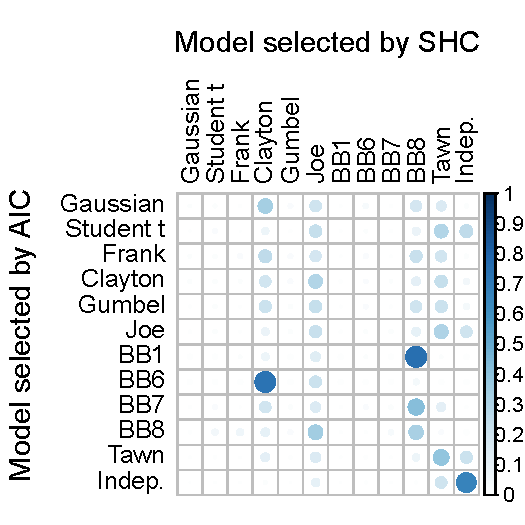
\includegraphics[scale=0.8]{copulas/splithalf_n250000_fig7AIC_SHC_}
	\end{subfigure}%
	\begin{subfigure}[t]{.48\textwidth}
		\centering
		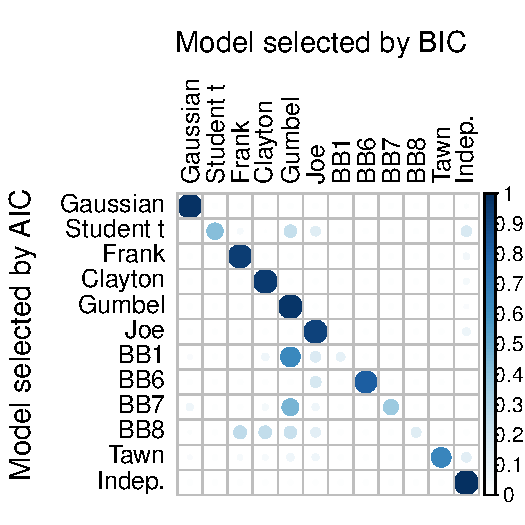
\includegraphics[scale=0.8]{copulas/splithalf_n250000_fig7AIC_BIC_}
	\end{subfigure}
	\caption{Left: How does SHC select models differently than AIC? Right:  How does BIC select models differently than AIC? Percentages are computed per row.}
	\label{fig:copulas-splithalf-plot-5}
\end{figure}


\subsection{Extrapolating Results to Larger Topic Set Sizes}

Similar to the case of the margins, we want to know if we underestimate or overestimate the goodness-of-fit of the copulas, and by how much. This is because, due to the inherent limitations of a split-half approach, we fit copulas on only 25 topics, as opposed to 50, since half of the data are used to provide an estimate of the ground truth. We follow an approach that is analogous to the one shown in Figure \ref{fig:diag5} to repeatedly split the data in three sets of topics. A set of 25 topics, a set of 50, and a set of 99 topics. The first two sets are used to fit two copula models respectively: $F_{25}^*$ and $F_{50}^*$. Using the final set of 99 topics as an estimate of the ground truth, we then compute a $\Delta_\text{obs}^{25}$ and $\Delta_\text{obs}^{50}$, respectively, for the two copula models.

In Figure \ref{fig:copulas-extrapolate-plot-1} we report the $\Delta_\text{obs}^{25}$ and $\Delta_\text{obs}^{50}$ values that we measured, in \num{150000} trials. All models were selected according to AIC. Overall, our results show that when models are fitted on 50 topics, as opposed to 25, they measure a $\Delta_\text{obs}$ that is slightly lower, which means that the goodness-of-fit of the copula models is underestimated. Moreover, we see that this occurrence is consistent across all copula families. These findings are consistent with the case of the margins. 

Table \ref{tab:copulas-extrapolate-table-1} shows that, on average, $\Delta_\text{obs}^{50}$ is only 2.6\% and 3.9\% smaller than $\Delta_\text{obs}^{25}$, for the case of AP and P@10 respectively. However, for the case of RR it is 10.3\% smaller, which is notable. 

In summary, these results show that our split-half approach tends to underestimate the goodness-of-fit of the copula models, only by a small amount. 

\begin{figure}[t]
	\centering	
	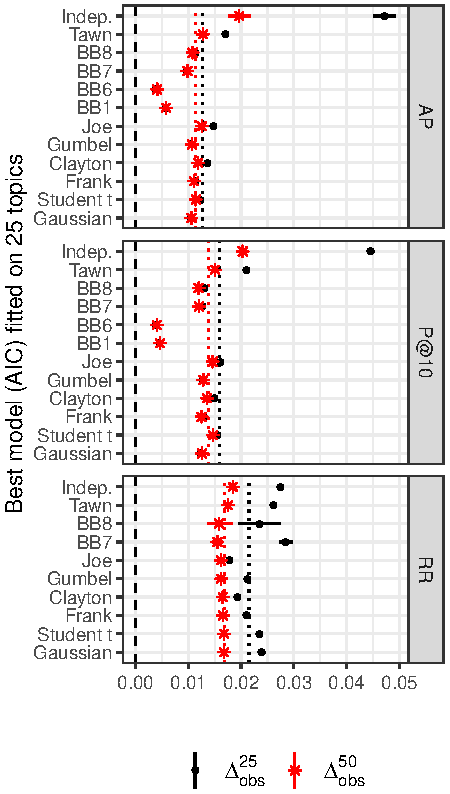
\includegraphics[scale=0.9]{copulas/extrapolate_n150000_fig1}
	\caption{How different would our $\Delta_\text{obs}$ measurements be, if the copula models had been fitted on 50 topics, as opposed to 25?.}
	\label{fig:copulas-extrapolate-plot-1}
\end{figure}

\begin{table}[!t]
	\centering
	\begin{tabular}{c c}
		% middle column is all italic
		\toprule
		& $\overline{\left(\frac{\Delta_\text{obs}^{50} - \Delta_\text{obs}^{25}}{\Delta_\text{obs}^{25}}\right)}$ \\ \midrule
		AP    & -0.026       \\
		P@10  & -0.039       \\
		RR    & -0.103      \\ \bottomrule
	\end{tabular}
	\caption{How different is $\Delta_\text{obs}^{50}$ compared to $\Delta_\text{obs}^{25}$?}
	\label{tab:copulas-extrapolate-table-1}
\end{table}

\subsection{Summary of Results}

Summarizing our results, we found that the copula models measure a $\Delta_{\text{obs}}$ that is about 23\% higher than our expectation, when they are selected by AIC. These results are somewhat worse compared to the case of the margins, but still within reason. We did not detect any obvious outliers.
 
Looking at the frequency with which each copula family is selected, we see that they are selected quite similarly, between the case of 25 and 50 topics.  
The Tawn copula gets selected with the highest frequency. Due to the fact that this is the only asymmetric family that is incorporated in the simulation, coupled with the fact that the distribution of per-topic score differences tends to be skewed; we speculate that the goodness-of-fit of the copulas would likely improve, if additional asymmetric families were included in the list of candidates. However, we leave this for future work.

Looking for ways of refining the quality of the models, we experimented with alternative ways of selecting them, including AIC, BIC, LL as well as our criterion (SHC), and found that our criterion improves the overall mean GoF, consistently across all effectiveness measures. The overall change over AIC (the next best criterion) is from around -0.23 to -0.19, which is notable. Moreover, the selections that SHC makes are significantly different from those of AIC, BIC or LL. Since a large selection of criteria was considered, it is likely that to further improve the goodness-of-fit, would require additional candidate copulas to be considered. 

In a separate, smaller scale experiment, we determined that our estimates regarding $\Delta_{\text{obs}}$ are underestimated by 2.6\%, 3.9\% and 10.3\% for AP, P@10 and RR respectively, which is quite low. 














